\chapter{序論}
欧州原子力研究機構(CERN)に設置されている大型ハドロン衝突型加速器(LHC)では、現在、素粒子物理の基礎となっている標準模型の精密測定や標準模型を超える物理現象の探索が行われている。ATLAS実験はLHC上にある1つの衝突点で行われている実験であり、設置しているATLAS検出器を用いて崩壊粒子の測定が行われている。LHCでは加速器のアップグレード(HL-LHC)を予定しており、これに向けてATLAS検出器のアップグレードを行う。この章ではLHC-ATLAS実験とそのアップグレード計画について説明する。

\section{LHCについて}
LHCはCERNの地下およそ100 $\rm{m}$に設置されている周長26.7 $\rm{km}$の大型ハドロン衝突型加速器である。
バンチと呼ばれる陽子のかたまりを7 $\rm{TeV}$まで加速し、衝突させる。世界最大エネルギーの加速器である。

陽子ビームの加速は4つの前段加速器を用いて行う。始めに水素ガス中の水素原子から電子を分離することで陽子を生成する。
その後最初の線形加速器(Linear Accelarator: LINAC)、陽子シンクロトロンブースター(Proton Synchrotron Booster: PSB)、陽子シンクロトロン(Proton Synchrotron: PS)、スーパー陽子シンクロトロン(Super Proton Synchrotron)で加速されたのちLHCに入射する。CERNにある加速器の概要を図\ref{LHC_overview}に示す。
LHCには4つの衝突点があり、それぞれALICE(A Large Ion Collider Experiment)、LHCb、CMS(Compact Muon Solenoid)、ATLAS(A
Troidal LHC Apparatus)実験が行われている。それぞれの衝突点には崩壊粒子の飛跡やエネルギーを測定するための検出器が設置されており、それら検出器で取得したデータを元に多様な物理解析が行われている。

\begin{figure}[bpt]\centering
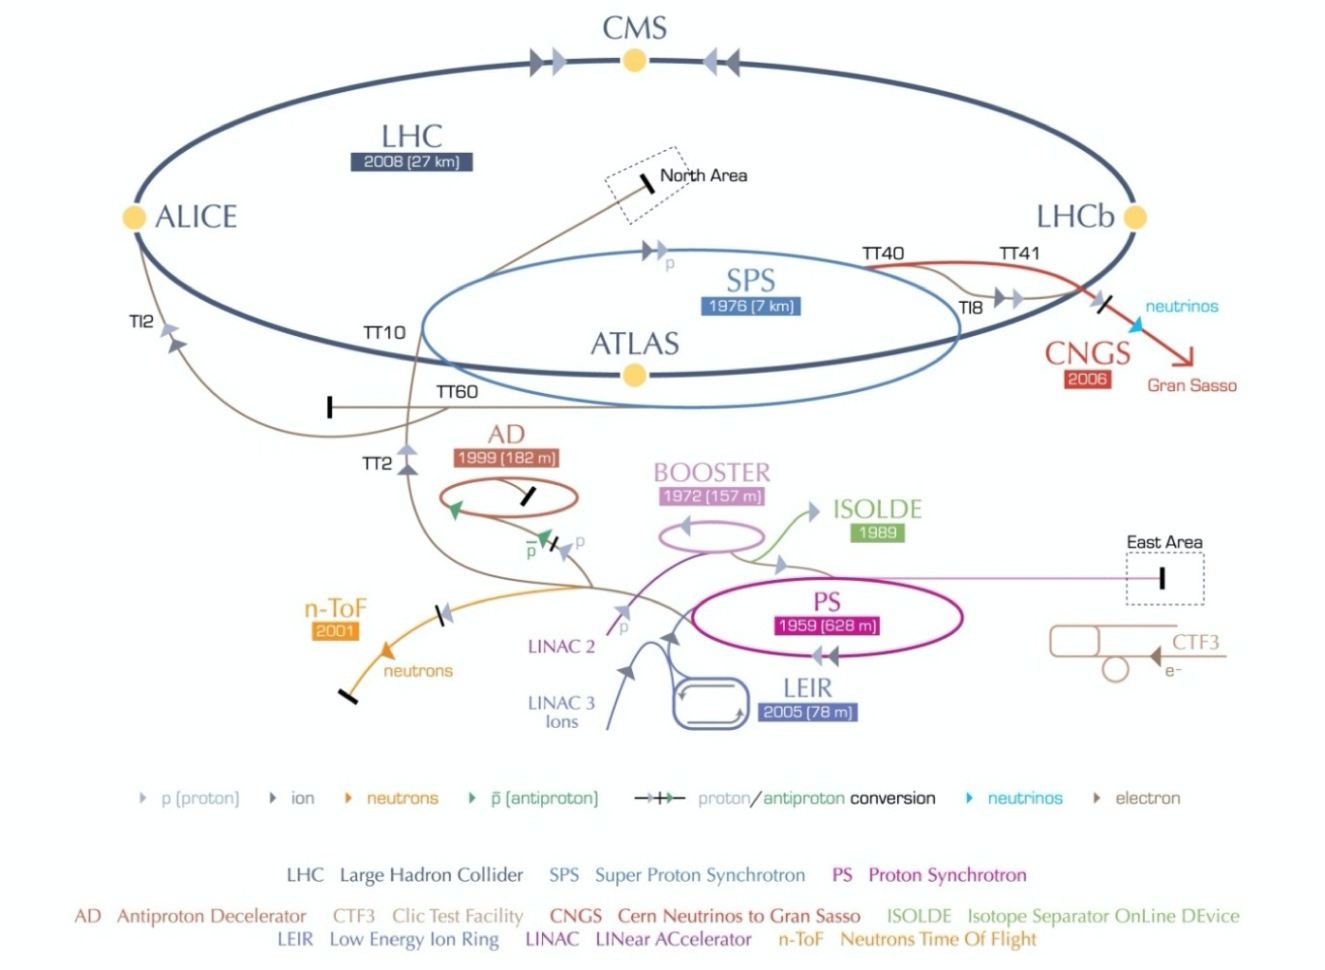
\includegraphics[width=12cm]{LHC_overview}
\caption[LHCの全体像]{LHCの全体像\cite{1-1}}
\label{LHC_overview}
\end{figure}

\section{ATLAS実験}
初めにATLAS実験に用いる座標系と用語について説明する。まず衝突点を原点として定義しており、ビーム軸を$z$軸、これに対して垂直な平面を$x-y$平面とする。
$x$軸方向は原点からみてLHCリングの中心に向かう方向であり、$y$軸は地上に向かう方向である。
方位角$\phi$は$z$軸周りの角度であり、極角$\theta$は$z$軸とのなす角である。大抵、極角$\theta$は以下のようにローレンツ不変量$\eta$で表される。
\bbb
\eta = -\rm{ln tan\left(\frac{\theta}{2}\right)}
\eee


\subsection{ATLAS検出器}
ATLAS検出器は複数の検出器から構成され、陽子の衝突によって生成された粒子の運動量、エネルギーを測定することができる。
最内装に内部飛跡検出器が設置されていて、次に超電導ソレノイド磁石、カロリメータ、トレノイド磁石、ミューオン検出器の順に設置されている。ビームパイプ以外をほとんど検出器で覆うようなデザインとなっている。
ATLAS検出器の全体図を図\ref{atlas_detector}に示す。

\begin{figure}[bpt]\centering
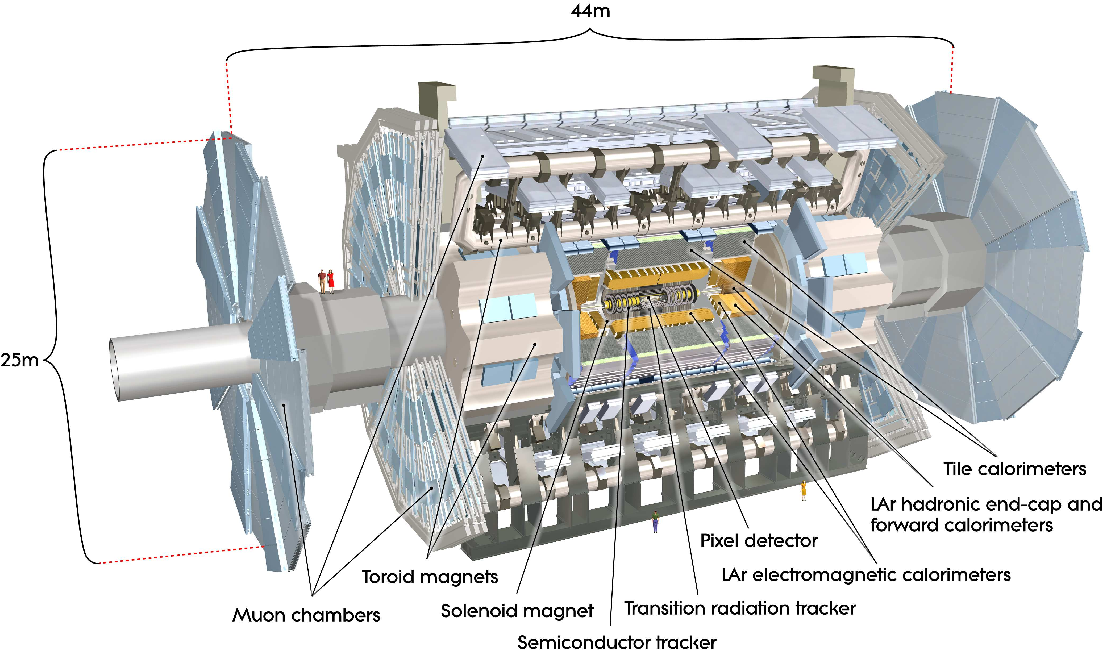
\includegraphics[width=10cm]{atlas_detector}
\caption[ATLAS検出器]{ATLAS検出器\cite{1-2}}
\label{atlas_detector}
\end{figure}

%\begin{figure}[bpt]\centering
%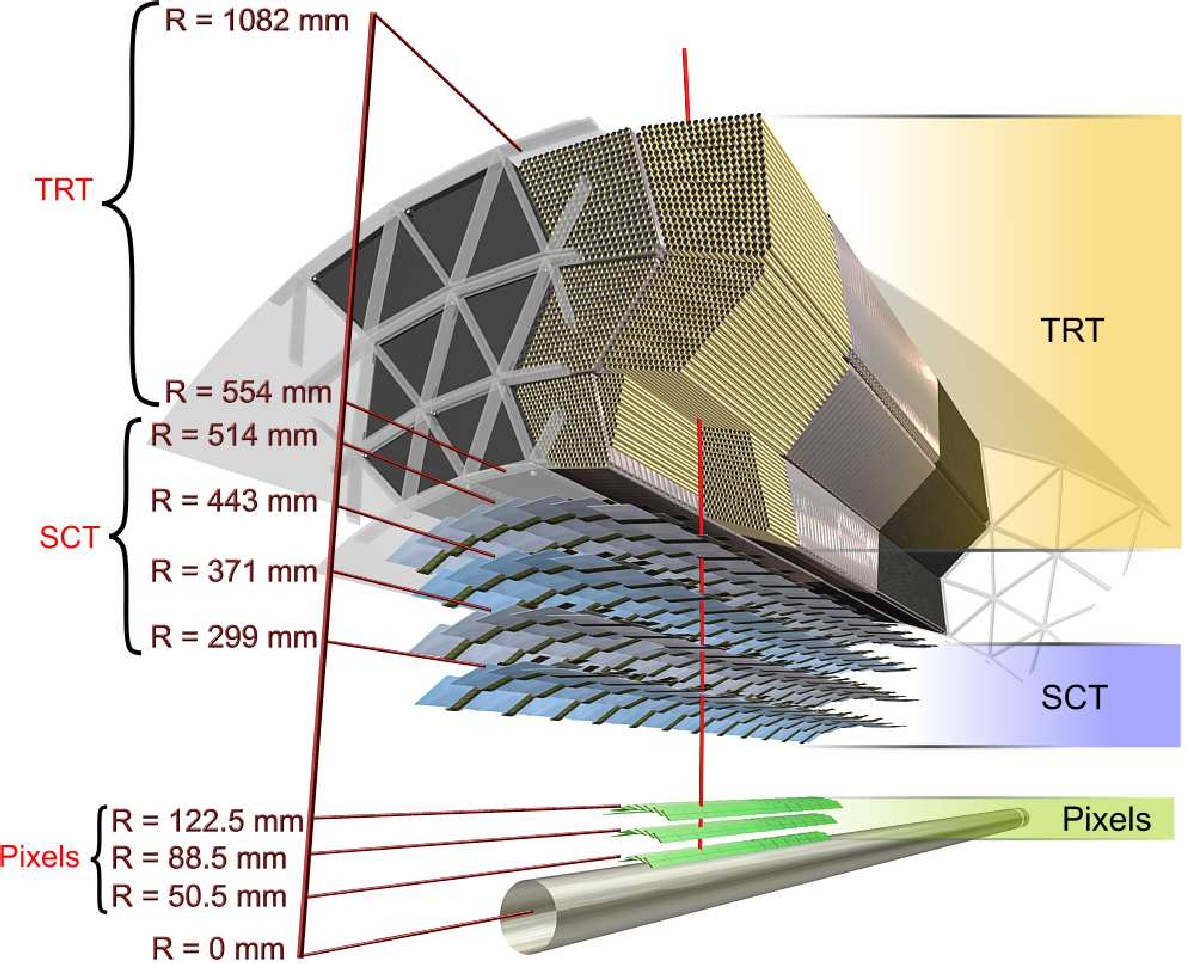
\includegraphics[width=10cm]{atlas_detector_cross_section}
%\caption[ATLAS検出器]{ATLAS検出器\cite{1-2}}
%\label{atlas_detector_cross_section}
%\end{figure}

\subsection{内部飛跡検出器}
ATLAS検出器の最内層に位置する検出器である。
内部飛跡検出器は粒子の飛跡を測定するための検出器であり、その曲がり具合から粒子の運動量を計算できる。
半径$1.15 \rm{m}$、長さ$7 \rm{m}$の円柱形であり、$|\eta|\leq 2.5$の領域を覆っている。超伝導ソレノイド磁石で2 $\rm{T}$の磁場が$z$方向にかけられる。この検出器はさらに3つの検出器で構成され、内側からピクセル検出器、ストリップ検出器、遷移放射検出器の順に設置されている。
ピクセル、ストリップ検出器は階層構造になっており、粒子は複数の検出器を通過する。通過位置をつなぎ合わせることで粒子の軌跡を計算することができる。

内部飛跡検出器の全体図を図\ref{inner_detector}に示す。

\begin{figure}[bpt]\centering
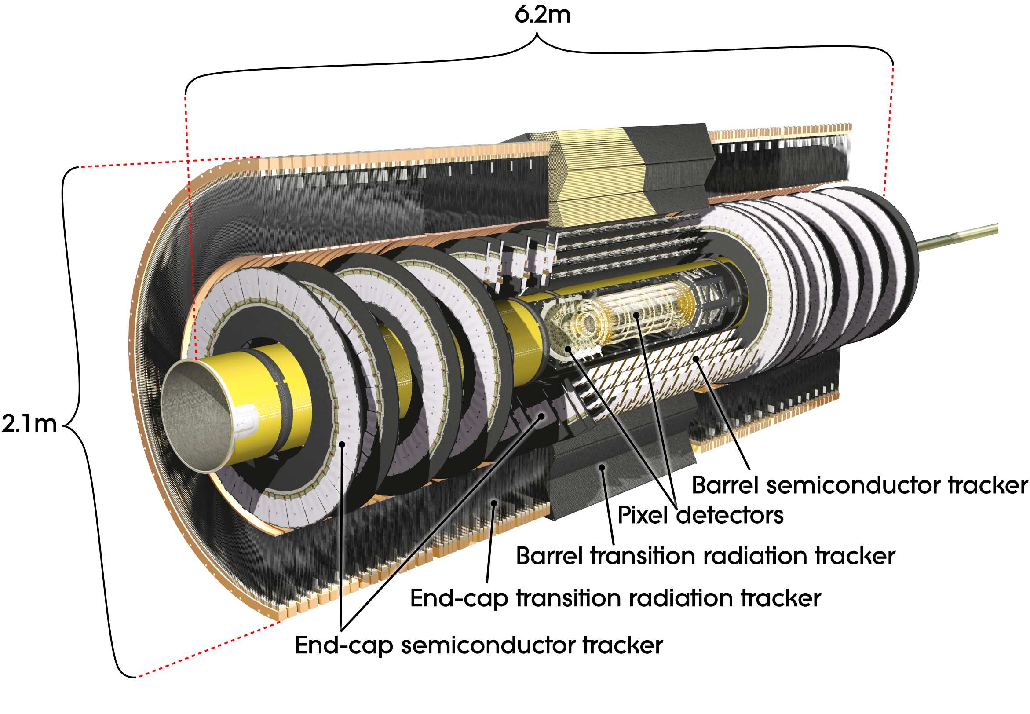
\includegraphics[width=10cm]{inner_detector}
\caption[内部飛跡検出器]{内部飛跡検出器\cite{1-2}}
\label{inner_detector}
\end{figure}


%検出器は$\eta$の範囲によってバレル部とエンドキャップ部に分かれる。図\ref{inner_cross_section}にビーム軸方向の端面図を示す。
%
%\begin{figure}[bpt]\centering
%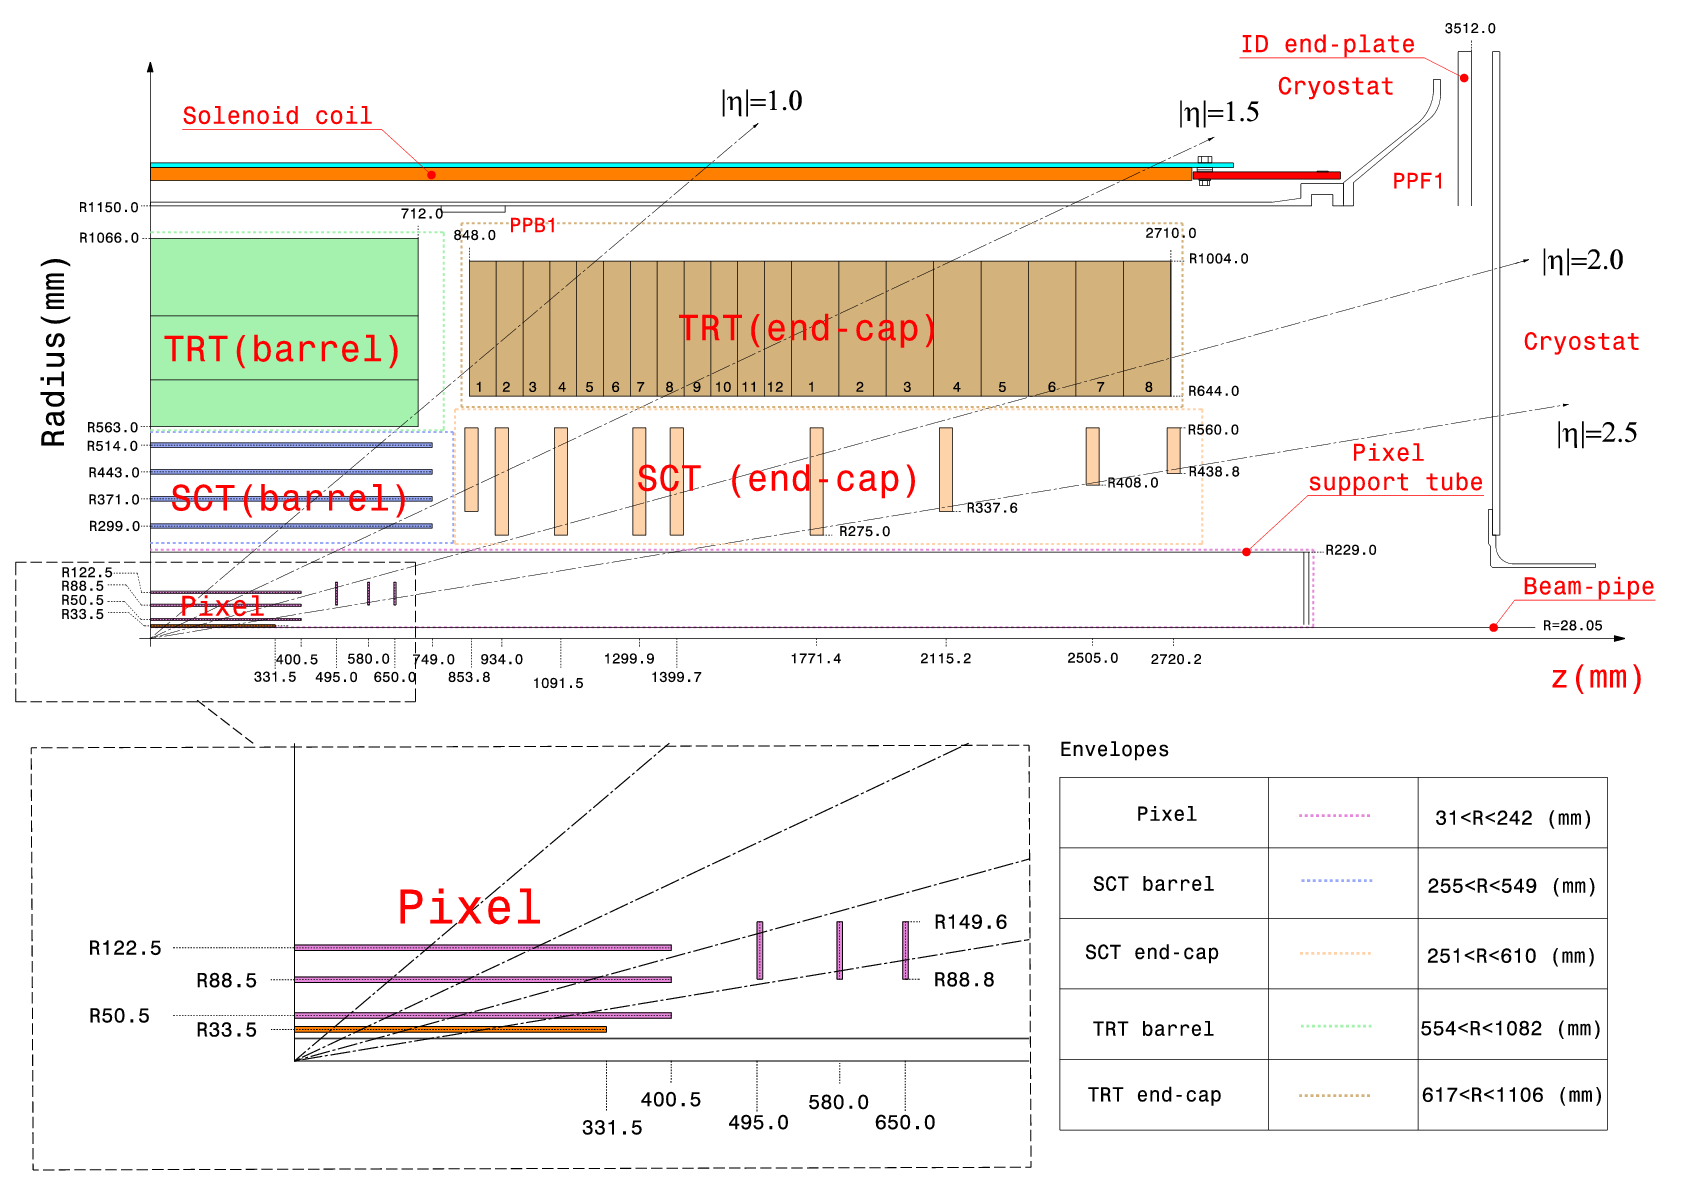
\includegraphics[width=12cm]{inner_cross_section}
%\caption[内部飛跡検出器]{内部飛跡検出器\cite{1-4}}
%\label{inner_cross_section}
%\end{figure}

\clearpage
\subsubsection{ピクセル検出器}

内部飛跡検出器の最内層に位置する検出器である。
ピクセル検出器はバレル層が4層、Diskと呼ばれるエンドキャップ層が6層で構成される。
バレル部の最内層はIBL(Insertable B-Layer)と呼ばれ、順にB-Layer、Layer-1、Layer-2となっている。

ピクセル検出器の全体図を図\ref{pixel_detector_overview}に示す。
\begin{figure}[bpt]\centering
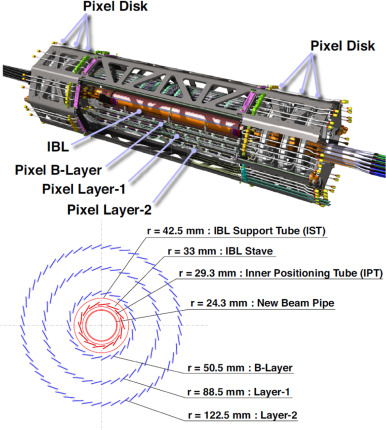
\includegraphics[width=10cm]{pixel_detector_overview}
\caption[ピクセル検出器全体]{ピクセル検出器全体\cite{1-5}}
\label{pixel_detector_overview}
\end{figure}

ピクセル検出器の各層は、モジュールと呼ばれる最小単位の検出器をいくつも搭載している。
ピクセルモジュールを図\ref{pixel_detector}に示す。
このピクセルモジュールの詳細については2章で述べる。
\begin{figure}[bpt]\centering
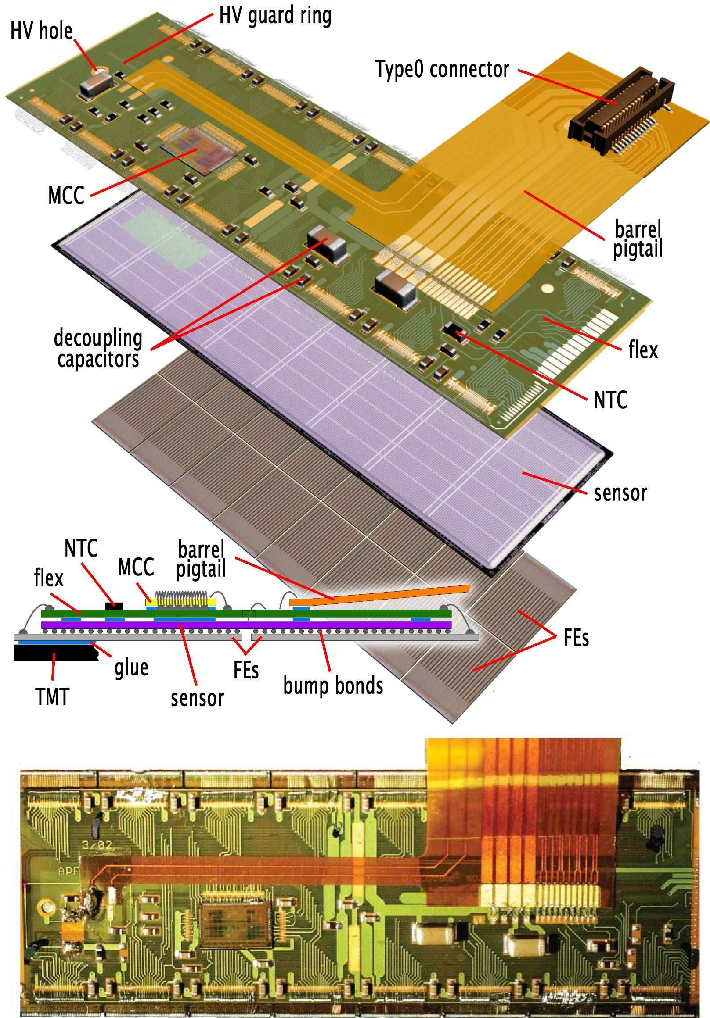
\includegraphics[width=8cm]{pixel_detector}
\caption[ピクセルモジュール]{ピクセルモジュール\cite{1-2}}
\label{pixel_detector}
\end{figure}


\clearpage
\section{HL-LHC実験アップグレード計画}
上述したように、LHCでは加速器のアップグレードを予定しており、これをHL-LHCアップグレード計画と呼ぶ。詳細を以下に示す。
\subsection{概要}
HL-LHCではルミノシティ呼ばれる陽子バンチの密度を上げることで、衝突確率を大きくし、取得統計数を増やす目的がある。
LHCとHL$-$LHCの比較を表\ref{compare_lhc}に示す。

\begin{table}[tbp]
\begin{center}
\caption[LHCの比較]{LHCの比較\cite{1-6}}
\label{compare_lhc}
  \begin{tabular}{|lll|} \hline
    & LHC & HL$-$LHC \\ \hline
    重心系エネルギー & 14 & 14 \\
    瞬間ルミノシティ[$\rm{cm^{-2}s^{-1}}$] & $1\times 10^{34}$ & $7\times10^{34}$ \\
    積分ルミノシティ[$\rm{fb^{-1}}$] & $300$ & $3,000$ \\
    1衝突あたりのイベント数 & $23$ & $138$ \\ \hline 
  \end{tabular}
\end{center}
\end{table}

LHCの運転計画を表\ref{hllhc_plan}に示す。
2020年8月地点の計画では、2025年の初めよりHL-LHCの導入が始まり、2027年の途中からHL-LHC運転開始の予定となっている。
\begin{figure}[bpt]\centering
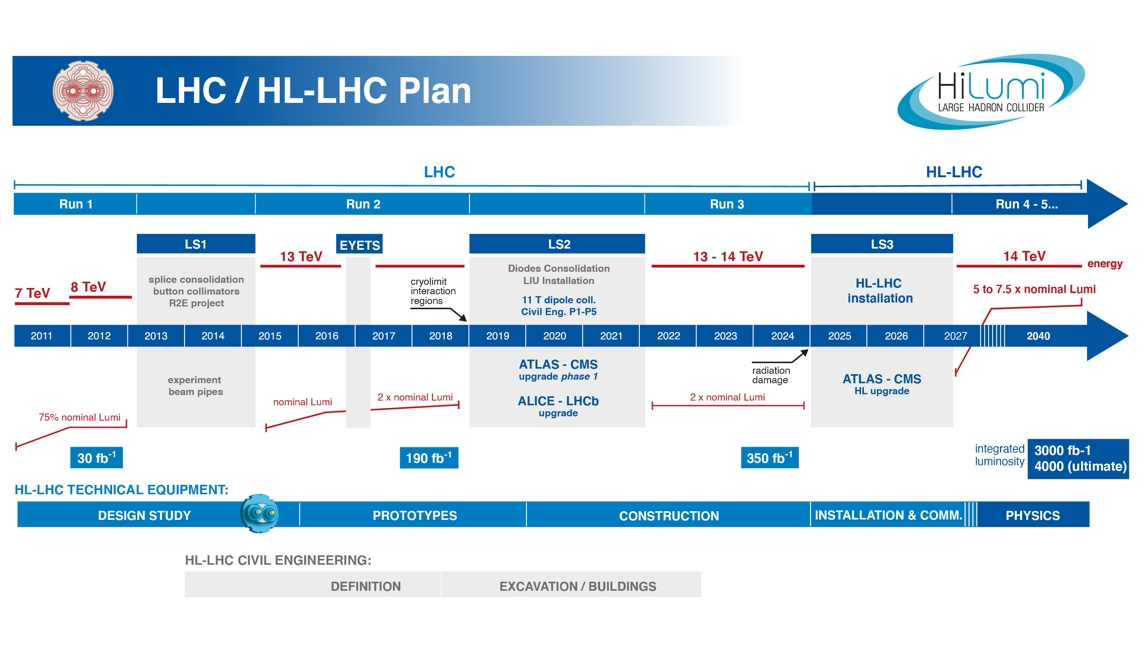
\includegraphics[width=12cm]{hllhc_plan}
\caption[HL-LHC運転計画]{HL-LHC運転計画\cite{1-7}}
\label{hllhc_plan}
\end{figure}

\subsection{内部飛跡検出器のアップグレード}
ルミノシティの増加に伴い、検出器には以下のような性能が要求される。
\begin{itemize}
  \item 放射線耐性の向上
  \item 高速読み出し
  \item 検出器の細密化
\end{itemize}

HL-LHCに向けてATLAS内部飛跡検出器はアップグレードを予定しており、上記の要求を満たすように開発を進めている。
アップグレード後の検出器をITk(Inner Tracker)と呼ぶ。イメージを図\ref{itk_image}に示す。

\begin{figure}[bpt]\centering
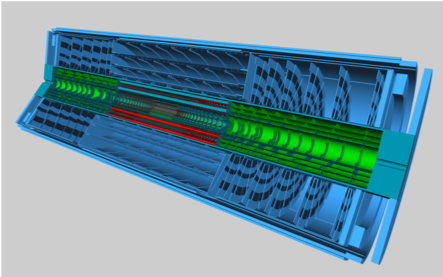
\includegraphics[width=10cm]{itk_image}
\caption[ITkのイメージ]{ITkのイメージ\cite{1-3}}
\label{itk_image}
\end{figure}

\clearpage
\subsubsection{ITkの構成と現行との比較}
図\ref{itk_cross_section}にITkのビーム軸方向の断面図を示す。
ITkはピクセル検出器とストリップ検出器で構成される。
ピクセル検出器はバレル、インクラインド、エンドキャップ部で構成され、バレル部は5層となっている。

\begin{figure}[bpt]\centering
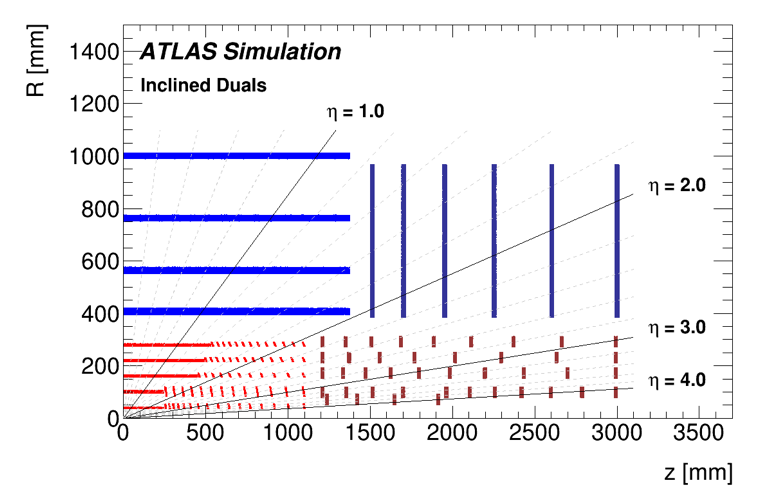
\includegraphics[width=10cm]{itk_cross_section}
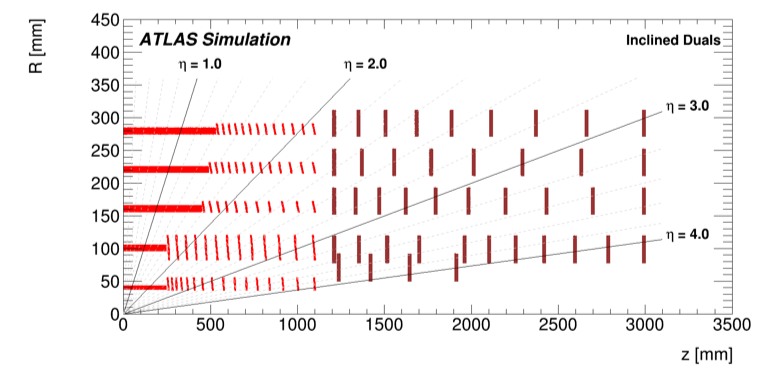
\includegraphics[width=10cm]{itk_pixel_cross_section}
\caption[ITkの断面図]{ITkの断面図\cite{1-3}}
\label{itk_cross_section}
\end{figure}

ピクセル検出器の配置に関して、現行とITkの比較を表\ref{compare_itk_pixel}に示す。
またモジュール数の比較を表\ref{compare_itk_modules}に示す。

\begin{table}[tbp]
\begin{center}
\caption[ピクセル検出器配置の比較]{ピクセル検出器配置の比較}
\label{compare_itk_pixel}
  \begin{tabular}{|lll|} \hline
    & 現行 & ITk \\ \hline
    $r[\rm{mm}]$ & $33~129$ & $39~279$ \\ 
    $|\eta|$ & $<2.5$ & $<4$ \\ 
    層の数 & 4 & 5 \\ \hline
  \end{tabular}
\end{center}
\end{table}

\begin{table}[tbp]
\begin{center}
\caption[ピクセルモジュール数の比較]{ピクセルモジュール数の比較}
\label{compare_itk_modules}
  \begin{tabular}{|l||ll|ll|ll|} \hline
          & バレル部 &            & インクラインド部 & & エンドキャップ部 & \\ \hline 
    層    & 現行     & ITk        & 現行& ITk          & 現行  & ITk \\ \hline
    1     & $280$    & $192$      & $-$ & $512$        & $-$   & $64$ \\ 
    2     & $286$    & $240$      & $-$ & $520$        & $-$   & $242$ \\ 
    3     & $494$    & $660$      & $-$ & $660$        & $-$   & $320$ \\ 
    4     & $676$    & $960$      & $-$ & $1040$       & $288$ & $352$ \\ 
    5     & $-$      & $1300$     & $-$ & $1300$       & $-$   & $468$ \\ \hline
    合計  & $1736$   & $3352$     & $0$ & $4032$       & $288$ & $1446$ \\ \hline\hline
  \end{tabular}
\end{center}
\end{table}

\subsection{期待される物理}
ITkは現行ピクセル検出器に比べカバーする$\eta$の範囲が大きい。
そのため前方方向に大きな運動量を持つ粒子が生じるような物理現象に対する感度が向上する。

このような物理現象の例として、ボゾン粒子結合によるヒッグス粒子生成過程(Vector boson fusion higgs production, \textbf{VBF})をあげる。
この過程のファインマン図及びイベントディスプレイを図\ref{VBF_image}に示す。
この衝突により生じる2つのクオークジェットは前方方向に大きい運動量を持つ。
ITkではこれらのジェットを正確に捉えることができ、VBFイベントの測定精度を向上することができる。
この測定における系統誤差は表\ref{VBF_uncertainty}のように見積もられる\cite{1-3}。

\begin{figure}[bpt]
  \begin{minipage}{0.4\hsize}
    \begin{center}
    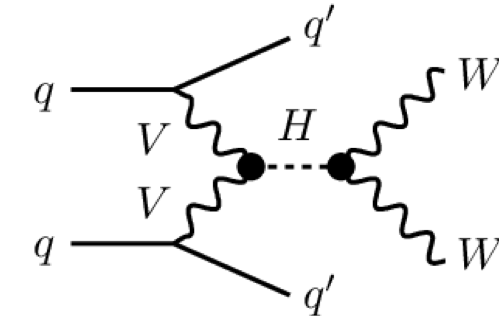
\includegraphics[width=60mm]{VBF_fainman}
    \end{center}
  \end{minipage}
  \begin{minipage}{0.4\hsize}
    \begin{center}
    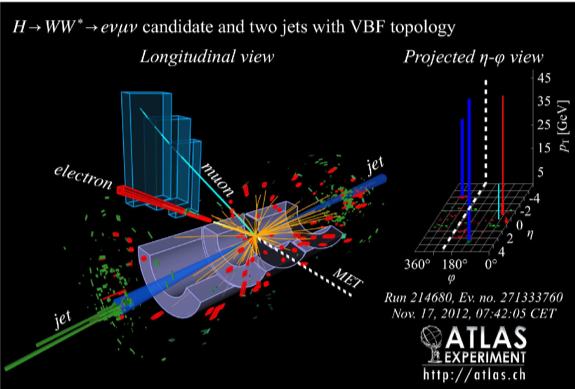
\includegraphics[width=60mm]{VBF_event_display}
    \end{center}
  \end{minipage}
  \caption[VBFイベントの図]{VBFイベントの図}
  \label{VBF_image}
\end{figure}

\begin{table}[tbp]
\begin{center}
\caption[VBFの測定における系統誤差の見積もり]{VBFの測定における系統誤差の見積もり}
\label{compare_itk_pixel}
  \begin{tabular}{|lll|} \hline
    使用範囲 & $|\eta| <2.7 $ & $|\eta| < 4.0 $ \\ \hline
    & 22$\%$ & 12$\%$ \\ \hline
  \end{tabular}
\end{center}
\end{table}

その他広い$\eta$による利点として、bタグ精度の向上、主崩壊イベント由来のジェットの選別精度の向上、$\tau$レプトン識別精度の向上が見込まれ、多くの物理現象において測定精度の向上が見込まれている。
